\chapter{Livello Host-to-Network}
\section{Definizione e tecnologie}
Il livello \textbf{H2N} risolve due problemi, quello delle interconnessioni fra due host e quello dello scambio di dati fra due host. Nello specifico il livello \textbf{Fisico} di occupa di connettere gli host con diversi mezzi di trasmissione, invece il livello \textbf{Data-Link} si occupa del framing, del controllo e della correzzione di errori e di inviare i \textbf{\textcolor{blue}{frame}} solo fra nodi della \textbf{LAN}.
Ci sono più tipi di trasmissione:
\begin{enumerate}
    \item \textbf{Broadcast:} comunicazione tra un singolo mittente e tutti gli altri nodi.
    \item \textbf{Multicast:} comunicazione tra un singolo mittente e un gruppo di destinatari.
    \item \textbf{Anycast:} comunicazione tra un singolo mittente e almeno un destinatario in un gruppo.
    \item \textbf{Unicast:} comunicazione tra un singolo mittente e un singolo destinatario.
\end{enumerate}

Il protocollo H2N è implementato nella \textbf{NIC (Netwrok Interface Card)}, tutti i dispositivi della rete per comunicare devono averne una.

\begin{boxDef}
\textbf{\textcolor{brown}{LAN:}} area fisicamente limitate a cui sono connessi uno o più dispotivi. Misurata in \textbf{$\frac{\text{Bit}}{s}$}. Tutte le tecnologie seguono lo standard \textbf{IEEE Standard 802}, come \textbf{Ethernet (IEEE 802.3)} e \textbf{WLAN (IEEE 802.11x)}.
\end{boxDef}

\section{Ethernet}
Creata a metà degli anni '70 da Bob Metcalfe, che propose Ethernet nella sua tesi di dottorato.

\begin{boxDef}
\textcolor{brown}{Ethernet:} metodo di trasmissione usato globalmente perchè economico ed efficente, funziona bene con i protocolli dello stack \textbf{TCP/IP}.
Connessione di tipo \textbf{broadcast}, quindi tutti sono collegati allo stesso canale di comunicazione e anche trasmissione di tipo \textbf{braodcast}, quindi quando viene inviato un messaggio nella \textbf{LAN}, tutti i nodi ad essa collegati lo ricevono.
\end{boxDef}

Gli host utilizzano un indirizzo hardware o indirizzo \textbf{MAC (Media Access Control)} per capire chi è il destinatario dei dati.

\begin{boxDef}
\textcolor{brown}{MAC:} indirizzo unico della \textbf{NIC} a \textbf{48 bit} che viene inserito nella ROM quando viene realizzata. La sua struttura è formata da:
\begin{itemize}
    \item 3 bytes (24 bit) $\rightarrow$ \textbf{Organizationally Unique Identifier (OUI)}, di solito il produttore della NIC.
    \item 3 bytes (24 bit) $\rightarrow$ \textbf{NIC ID}, all'interno dell'OUI.
\end{itemize}
Ogni dispostivo per fare parte della LAN deve avere una NIC e quindi avrà anche un indirizzo MAC unico.
\end{boxDef}

L'indirizzo broadcast è FF-FF-FF-FF-FF-FF.

\newpage
Quindi:
\begin{itemize}
    \item Quando un host desidera trasmettere un pacchetto, inserisce l'indirizzo MAC del destinatario e lo trasmette nella LAN.
    \item Se l'indirizzo di destinazione del pacchetto corrisponde all'indirizzo MAC dell'host ricevente, quest'ultimo accetta il pacchetto e lo inoltra al protocollo successivo.
    \item Se l'indirizzo di destinazione non corrisponde all'indirizzo MAC dell'host ricevente, quest'ultimo scarta il pacchetto.
\end{itemize}

\vspace*{0.02\textheight}
\textbf{ESEMPIO:}
\begin{bashbox}
ddonati@linux > ifconfig eth0
eth0 Link encap:Ethernet HWaddr 00:10:5A:9D:88:AF
inet addr:192.168.1.3 Bcast:192.168.1.255 Mask:255.255.255.0
UP BROADCAST RUNNING MULTICAST MTU:1500 Metric:1
RX packets:92 errors:0 dropped:0 overruns:0 frame:0
TX packets:52 errors:0 dropped:0 overruns:0 carrier:0
collisions:0 txqueuelen:1000
RX bytes:14162 (13.8 KiB) TX bytes:6744 (6.5 KiB)
Interrupt:9 Base address:0xfc00
\end{bashbox}

\textcolor{red}{00:10:5A:9D:88:AF} è l'indirizzo MAC, invece, \textcolor{red}{192.168.1.3} è l'indirizzo IP.

\subsection{Frame Ethernet}
I pacchetti scambiati al livello host to netwrok sono chiamati \textbf{frame}. Per tecnologie e topologie diverse, il formato di ogni frame è sempre lo stesso.

\begin{figure}[!htb]
    \centering
    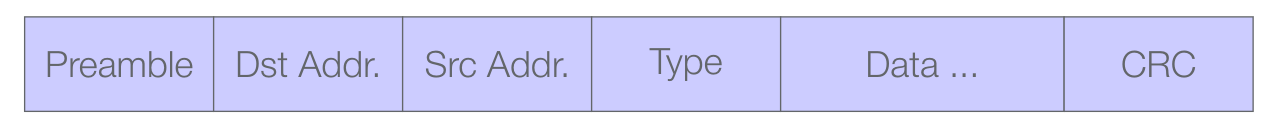
\includegraphics[width=0.9\linewidth]{Images/host_to_network/h2n.png}
    \caption{Frame Ethernet.}
\end{figure}

\subsection{Preamble}
Campo da 8 byte, di cui i primi 7 byte valgono tutti 10101010 e l'ultimo byte vale 10101011. 
I primi 7 byte servono per attivare e sincronizzare i ricevitori, due 1 consecutivi nell'ultimo byte indicano che la sincronizzazione è finita e il contenuto del frame sta per arrivare.

\subsection{Indirizzo di Destinazione e di Origine}
Due campi da 6 byte ciascuno, che indicano l'indirizzo MAC di destinazione e l'indirizzo MAC di origine. Quando un ricevitore riceve un MAC equivalente al suo passa il contenuto al layer di Rete, altrimenti lo scarta.

\subsection{Tipo}
Campo da 2 byte che indica il tipo di protocollo che verrà usato p al layer di Rete (IP, Nevel IPX, Apple Talk, ecc), è usato anche per supportare i protocolli \textbf{ARP} e \textbf{RARP}.

\subsection{Data e Dimensione}
Contiene i dati (\textbf{IP Datagram}), l'unità massima di trasmissione per Ethernet (\textbf{MTU}) è 1500 byte, altrimenti va frammentato, invece, quella minima è 46 byte, se minore di questa cifra va aggiuntoun padding.

\subsection{CRC (Cyclic Redundancy Check)}
Campo da 4 byte che consente all'adattatore che riceve i dati di rilevare la presenza di un errore nei bit del frame ricevuto.

\section{Protocollo ARP}
L'indirizzo IP non è riconosciuto dall'hardware, quindi il protocollo ARP si occupa di trasformare l'IP di un host nella stessa sua LAN nel suo corrispettivo indirizzo MAC.
Nello specifico usa due tipi di messaggi:
\begin{enumerate}
    \item Messaggio broadcast di richiesta con l'indirizzo IP.
    \item Messaggio unicast di risposta con il corrispettivo indirizzo MAC.
\end{enumerate}

\begin{figure}[!htb]
    \centering
    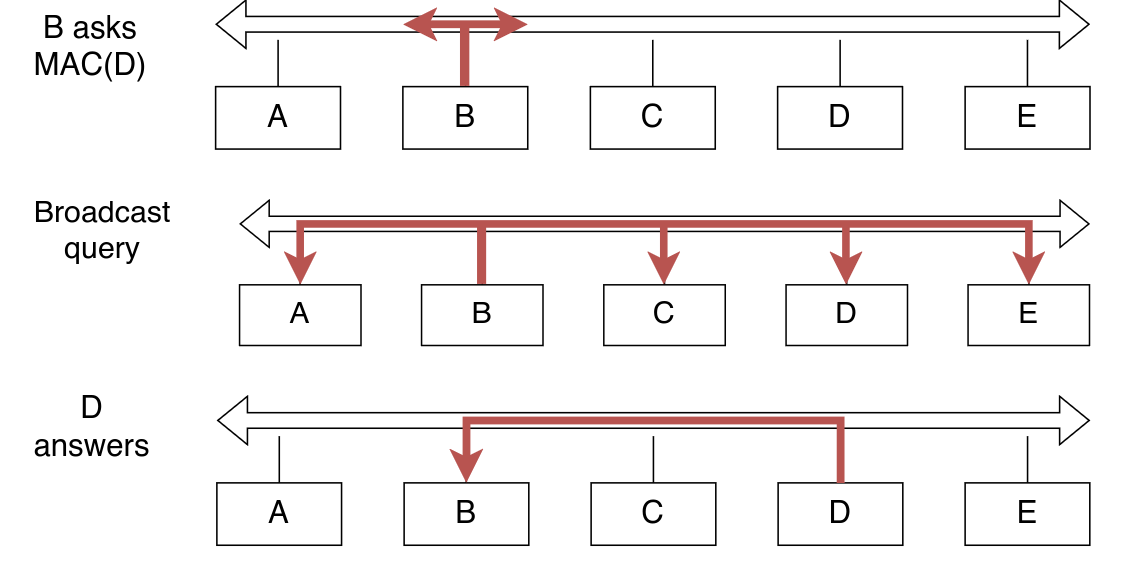
\includegraphics[width=0.7\linewidth]{Images/host_to_network/ARP.png}
    \caption{Protocollo ARP.}
\end{figure}

\subsection{ARP Cache}
Per ridurre il traffico di rete causato dallo scambio di messaggi ARP, ogni host memorizza temporaneamente nella cache le risoluzioni IP/MAC nella propria tabella. 

\begin{center}
\begin{tabular}{ ||c|c|c|| }
 \hline
 \textbf{IP} & \textbf{MAC} & \textbf{TTL} \\ 
 \hline
 \hline
 222.222.222.221 & 88:B2:2F:54:1A:0F & 13:45:00 \\ 
 \hline
 222.222.222.223 & 5C:66:AB:90:75:B1 & 13:52:00 \\ 
 \hline
\end{tabular}
\end{center}

\vspace*{0.02\textheight}
\textbf{ESEMPIO:}
\begin{bashbox}
ddonati@linux > sudo arp
Address HWtype Hwaddress Flags Mask Iface
ns1.ing.unimo.it ether 00:01:03:11:6B:63 C eth0
info-gw.ing.unimo.it ether 00:0A:57:05:A0:00 C eth0

donati@linux > ping brandy.ing.unimo.it
[...]

donati@linux > sudo arp
Address HWtype Hwaddress Flags Mask Iface
brandy.ing.unimo.it ether 00:11:11:5A:EB:41 C eth0
ns1.ing.unimo.it ether 00:01:03:11:6B:63 C eth0
info-gw.ing.unimo.it ether 00:0A:57:05:A0:00 C eth0
\end{bashbox}

\subsection{RARP}
Per ottenere l'indirizzo IP a partire da un indirizzo MAC si può usare il protocollo RARP, che funziona con la stessa struttura e nello stesso modo del protocollo ARP.

\newpage
\section{Interconnessione fra LAN}
Nel fare delle reti LAN molti grandi, possono causarsi molti problemi, dalle collisioni a il limite di lunghezza dello standard 802.3. 
\\
Per questo ci sono diversi tipi di dispositivi di rete, che dipendono da topologia, numero di host connessi, ecc:
\begin{itemize}
    \item \textbf{Hub.}
    \item \textbf{Brigde.}
    \item \textbf{Switch.}
    \item \textbf{L3 Switch.}
\end{itemize}

\subsection{Hub}
Dispositivo di livello fisico con due o più interfacce. Ripete i bit ricevuti su un'interfaccia a tutte le altre interfacce, ogni nodo connesso costituisce un segmento LAN.

\subsection{Bridge}
Dispositivo che opera a livello 2 nell'Ethernet frame, analizza l'header e distribuisce selettivamente in base al MAC di destinazione. Per trasmettere usa il protocollo CSMA/CD.

\subsection{Hub VS Bridge}
Il Bridge è più intelligente di un Hub, dato che è in grado di analizzare gli header e leggere il MAC, quindi, usando delle funzioni da filtro.
Inoltre, è utile perchè elimina le collisioni di dominio, aumenta il throughtput e non necessita di cambiamenti sugli host.
I bridge apprendono quali host sono raggiungibili tramite quali interfacce, infatti:
\begin{enumerate}
    \item Mantengono tabelle di filtro create automaticamente senza la necessità dell'intervento degli amministratori di rete.
    \item Quando viene ricevuto un frame, il bridge apprende la posizione del mittente.
    \item Registra la posizione del mittente nella tabella di filtro usando:
    \begin{itemize}
        \item Indirizzo MAC dell'host.
        \item Interfaccia del bridge.
        \item Time-To-Live (TTL).
    \end{itemize}
\end{enumerate}
I record obsoleti nella tabella di filtro vengono scartati in base alla scadenza del TTL.

\vspace*{0.02\textheight}
\textbf{ESEMPIO:}
\begin{bashbox}
iif frame.destination in filter_table then
    dest_lan_segment = lookup_filter_table(frame.destination)
    forward_to_lan_segment(frame, dest_lan_segment)
else
    {send frame to all ports except incoming port}
    flood(frame)
endif
\end{bashbox}

\subsection{Switch}
Si tratta di bridge ad alte prestazioni con numerose interfacce.
Ci sono più interfacce eterogenee (10/100/1000 Mbps) condivise e dedicate, senza collisioni con accesso dedicato e full duplex.

\subsection{Bridge VS Switch}
Concettualmente sono lo stesso dispositivo, il bridge è software, lo switch è hadrware.

\newpage
\subsection{Brigde in Linux}
\begin{figure}[!htb]
    \centering
    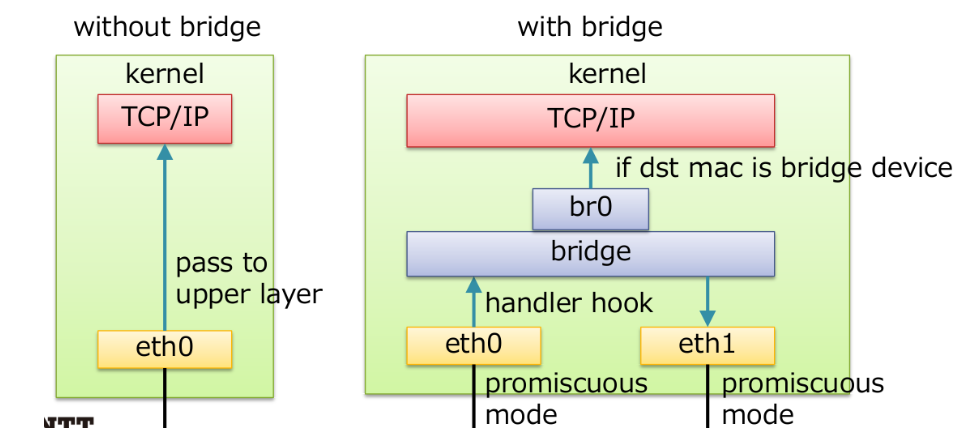
\includegraphics[width=0.7\linewidth]{Images/host_to_network/Bridge.png}
    \caption{Bridge in Linux.}
\end{figure}

I bridge possono essere configurati tramite il file \textbf{/etc/network/interfaces} oppure:

\vspace*{0.02\textheight}
\textbf{Creazione Bridge:}
\begin{bashbox}
bbrctl addbr <bridge>
ip link add <bridge> type bridge ...
\end{bashbox}

\vspace*{0.02\textheight}
\textbf{Aggiungere intefaccie al Bridge:}
\begin{bashbox}
bbrctl addif <bridge> <iface>
ip link set <iface> master <bridge>
\end{bashbox}

\vspace*{0.02\textheight}
\textbf{Vedere i Bridge configurati:}
\begin{bashbox}
bbrctl show <bridge>
\end{bashbox}

\vspace*{0.02\textheight}
\textbf{Vedere la lista dei MAC conosciuti dal Bridge:}
\begin{bashbox}
bbrctl showmacs <bridge>
\end{bashbox}

\newpage
\section{Virtual LAN}
Lo standard 802.1Q definisce le specifiche per definire più reti locali virtuali (VLAN) distinte, utilizzando la stessa infrastruttura fisica. Ogni VLAN agisce come se fosse separata dalle altre:
\begin{itemize}
    \item I pacchetti broadcast sono confinati all'interno della VLAN.
    \item Le comunicazioni a livello 2 sono confinate all'interno della VLAN.
    \item Le VLAN non possono comunicare fra di loro, se non a livello 3 tramite routing.
\end{itemize}
Le VLAN hanno diversi vantaggi tra cui:
\begin{enumerate}
    \item \textcolor{blue}{\textbf{Risparmio:}} evitano di dover creare nuove infrastrutture fisiche.
    \item \textcolor{blue}{\textbf{Performance:}} evita che i frame vengano inviati a destinazioni che non devono riceverli.
    \item \textcolor{blue}{\textbf{Security:}} un utente connesso a una VLAN non ha modo di vedere le altre.
    \item \textcolor{blue}{\textbf{Flessibilità:}} il movimento fisico di un utente non richiede dei cambiamenti fisici ma logici.
\end{enumerate}

Per porter funzionare e quindi riconoscere le VLAN bridge e switch devono essere conformi allo standard 802.1Q.
Devono essere in grado di fare queste tre azioni:
\begin{enumerate}
    \item \textbf{Ingresso:} il bridge deve saper riconoscere a quale VLAN appartiene il frame che arriva da una porta.
    \item \textbf{Trasmissione:} il bridge deve conoscere quale porta il frame deve essere trasmesso, in base alla VLAN alla quale appartiene.
    \item \textbf{Uscita:} il bridge deve essere in grado di far uscire il frame in modo che la sua VLAN venga riconosciuta da altri bridge.
\end{enumerate}
Le Untagged VLAN (private), dove a ogni porta appartiene una VLAN, non richiedono la conformità allo standard 802.1Q, ma solo che lo switch supporti la sua configurabilità.

\subsection{Tagged VLAN}
Lo standard 802.1Q permette di condividere lo stesso accesso fisico e che il bridge sia in grado di riconoscere le varie VLAN. Per questo, sono stati aggiunti 4 byte al frame Ethernet, per speicificare i dati della VLAN:
\begin{itemize}
    \item \textbf{TPI (Tag Protocol Identifier):} due byte, di valore 81 00, che indentifcano il protocollo 802.1Q.
    \item \textbf{TCI (Tag Control Information):} due byte che specificano le informazioni sul tag:
    \begin{itemize}
        \item I primi tre \textbf{(user priority)} indicano la priorità del frame.
        \item Il quarto bit \textbf{(CFI)} se è 1 indica che il frame viene da una token ring LAN.
        \item I restanti dodici bit \textbf{(VID} indica il tag (da 0 a 4095). Il tag 0 e il tag 4095 sono riservati e non possono essere usati.
    \end{itemize}
\end{itemize}

\begin{figure}[!htb]
    \centering
    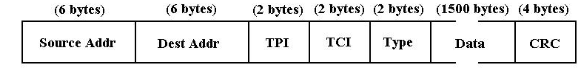
\includegraphics[width=0.7\linewidth]{Images/host_to_network/FrameVLAN.png}
    \caption{Frame standard 802.1Q.}
\end{figure}

\begin{figure}[!htb]
    \centering
    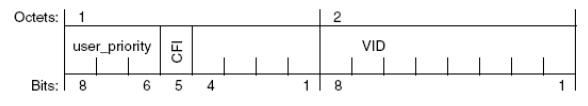
\includegraphics[width=0.7\linewidth]{Images/host_to_network/TCI.png}
    \caption{Campo TCI.}
\end{figure}

